
\label{prob:prob1}
Consider the initial boundary value problem
\begin{align*}
	u_{tt} &= u_{xx}, \\
	u(0,t) &= u(1,t) = 0, \\
	u(x,0) &= \sin(2 \pi x),\\
	u_t(x,0) &= 0.
\end{align*}
Numerically approximate the solution $u(x,t)$ for $t \in \left[0,.5\right]$.
Use $J=50$ subintervals in the $x$ dimension and $M=50$ subintervals in the $t$ dimension.
Animate the results.
Compare your results with the analytic solution $u(x,t) = \sin{(2 \pi x)} \cos{(2 \pi t)}$.
This function is known as a standing wave.
See Figure \ref{fig:prob1}.

\begin{figure}[H]
\centering
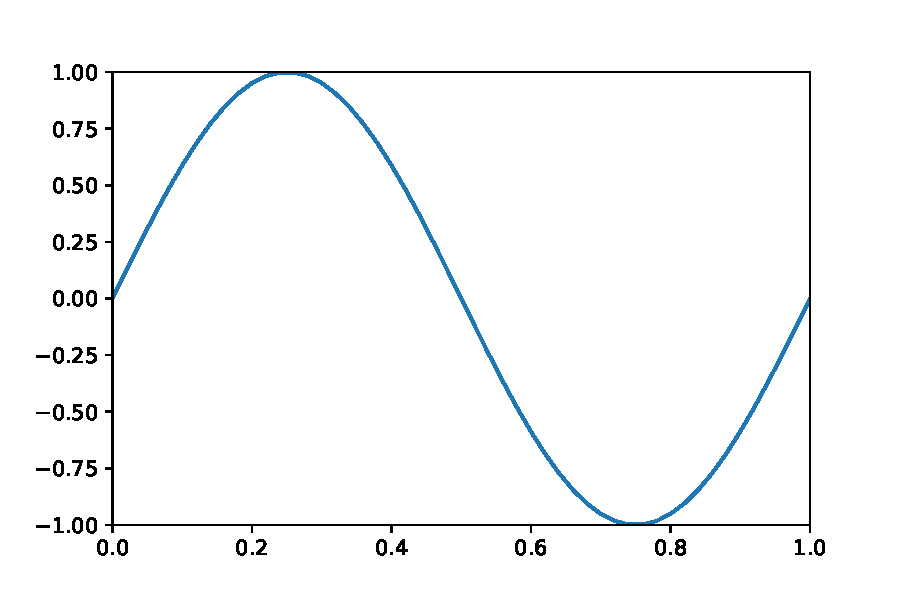
\includegraphics[width=\textwidth]{prob1.pdf}
\caption{$u(x,t=0)$.}
\label{fig:prob1}
\end{figure}

\label{prob:prob2}
Consider the initial boundary value problem
\begin{align*}
	u_{tt} &= u_{xx}, \\
	u(0,t) &= u(1,t) = 0, \\
	u(x,0) &= .2e^{-m^2(x-1/2)^2}\\
	u_t(x,0) &= .4m^2(x-1/2)e^{-m^2(x-1/2)^2}.
\end{align*}
The solution of this problem is a Gaussian pulse.
It travels to the right at a constant speed.
This solution models, for example, a wave pulse in a stretched string.
Note that the fixed boundary conditions reflect the pulse back when it meets the boundary.

Numerically approximate the solution $u(x,t)$ for $t \in \left[0, 1\right]$.
Set $m=20$.
Use 200 subintervals in space and 220 in time, and animate your results.
Then use 200 subintervals in space and 180 in time, and animate your results.
Note that the stability condition is not satisfied for the second mesh.
See \ref{fig:prob2}.

\begin{figure}[H]
\centering
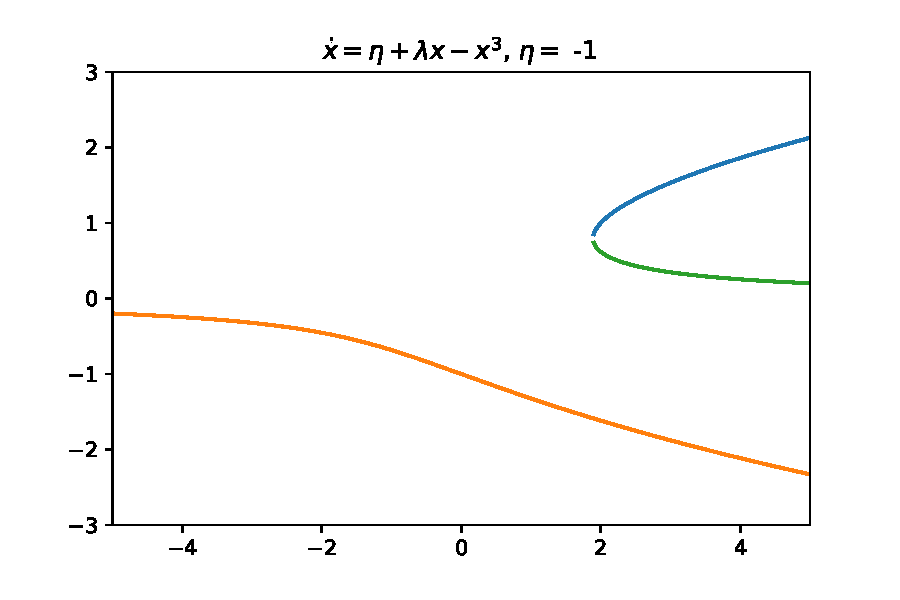
\includegraphics[width=\textwidth]{prob2.pdf}
\caption{$u(x,t=0)$.}
\label{fig:prob2}
\end{figure}

\label{prob:prob3}
Consider the initial boundary value problem
\begin{align*}
	u_{tt} &= u_{xx}, \\
	u(0,t) &= u(1,t) = 0, \\
	u(x,0) &= .2e^{-m^2(x-1/2)^2}\\
	u_t(x,0) &= 0.
\end{align*}
The initial condition separates into two smaller, slower-moving pulses, one travelling to the right and the other to the left.
This solution models, for example, a plucked guitar string

Numerically approximate the solution $u(x,t)$ for $t \in \left[0,2\right]$.
Set $m=20$.
Use 200 subintervals in space and 440 in time, and animate your results.
It is rather easy to see that the solution to this problem is the sum of two travelling waves, one travelling to the left and the other to the right, as described earlier.

\label{prob:prob4}
Consider the initial boundary value problem
\begin{align*}
	u_{tt} &= u_{xx}, \\
	u(0,t) &= u(1,t) = 0, \\
	u(x,0) &= \begin{cases} 1/3 & \text{if } 5/11 < x < 6/11,\\
	0 & \text{otherwise}
	\end{cases}\\
	u_t(x,0) &= 0.
\end{align*}

Numerically approximate the solution $u(x,t)$ for $t \in \left[0, 2\right]$.
Use 200 subintervals in space and 440 in time, and animate your results.
Even though the method is second order and stable for this discretization, since the initial condition is discontinuous there are large dispersive errors.
See Figure \ref{fig:prob4}.

%\begin{figure}[H]
%\centering
%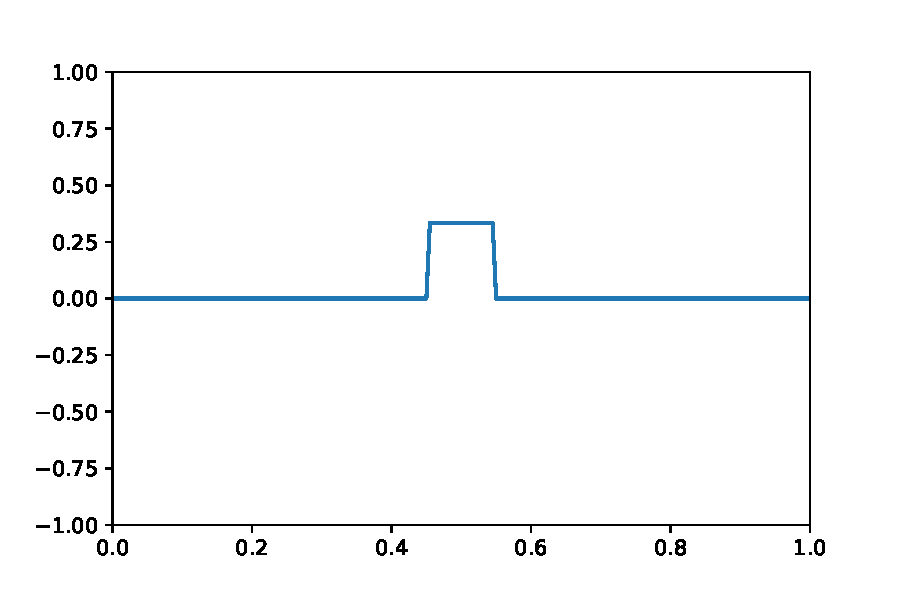
\includegraphics[width=\textwidth]{prob4.pdf}
%\caption{$u(x,t=0)$.}
%\label{fig:prob4}
%\end{figure}
%
\label{prob:prob5}
Numerically solve the initial value problem
\begin{align*}
	&{ } u_t -su_x + uu_x = u_{xx}, \quad x \in (-\infty,\infty),\\
	&{ } u(x,0) = v(x),
\end{align*}
for $t \in [0,1]$.
Let the perturbation $v(x)$ be given by
\[v(x) = 3.5(\sin{(3x)} + 1)\frac{1}{\sqrt{2\pi}} \exp{(-x^2/2)}\]
And let the initial condition be $u(x, 0) = \hat{u}(x) + v(x)$
Approximate the $x$ domain,$(-\infty, \infty)$, numerically by the finite interval $[-20,20]$, and fix $u(-20) = u_-$, $u(20) = u_+$. Let $u_- = 5$, $u_+ = 1$.
Use 150 intervals in space and 350 steps in time.
Animate your results.
You should see the solution converge to a translate of the travelling wave $\hat{u}$.
See Figure \ref{fig:prob5}.

Hint: This difference scheme is no longer a linear equation.
We have a nonlinear equation in $U^{n+1}$.
We can still solve this function using Newton's method or some other similar solver.
In this case, use \li{scipy.optimize.fsolve}.

\begin{figure}[H]
\centering
\begin{subfigure}{.49\textwidth}
\centering
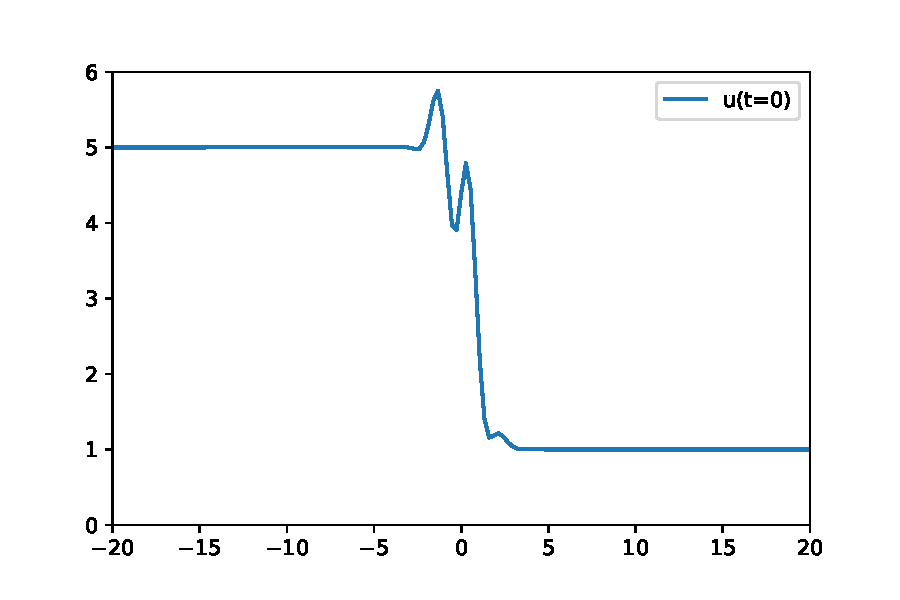
\includegraphics[width=\linewidth]{prob5_initial.pdf}
\caption{$u(x,t=0)$.}
\end{subfigure}
%
\begin{subfigure}{.49\textwidth}
\centering
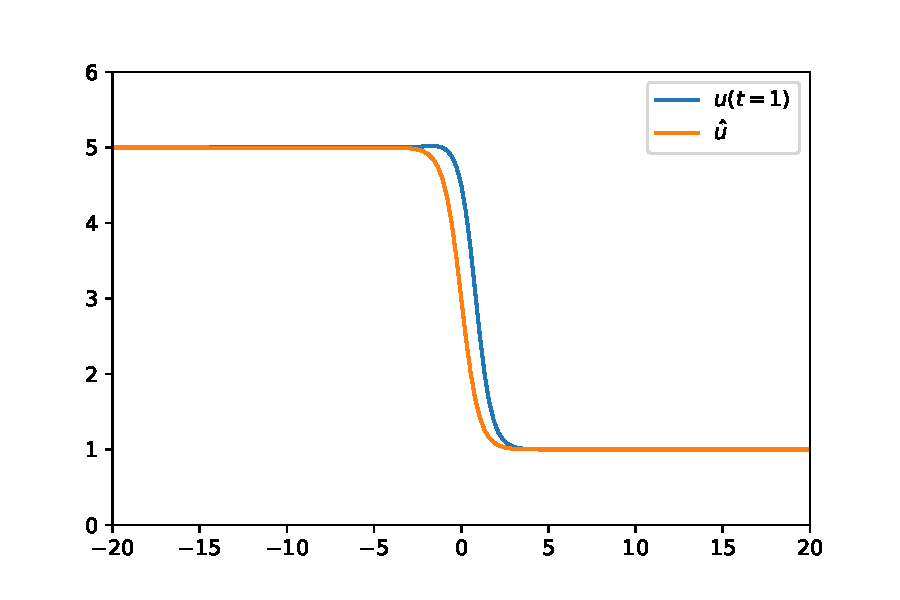
\includegraphics[width=\linewidth]{prob5_ufinal_utilda.pdf}
\caption{$u(x,t = 1)$ vs $\hat{u}$.}
\end{subfigure}
\caption{The graphs for Problem \ref{prob:prob5}}
\label{fig:prob5}
\end{figure}
